\documentclass[11pt,a4paper]{article}
\usepackage[margin=1in]{geometry}
\usepackage{booktabs}
\usepackage{graphicx}
\usepackage{hyperref}
\usepackage{float}
\usepackage{caption}
\usepackage{setspace}
\setstretch{1.1}

\title{AI651 Assignment 1\\Task 1 Report}
\author{Talha Tahir Qureshi\\Lahore University of Management Sciences}
\date{Fall 2026}

\begin{document}
\maketitle

\noindent\textbf{GitHub repository (public):}
\url{https://github.com/ttqureshi/DL4STG-PA1}

\vspace{0.5em}
\noindent\textbf{Run setting used for all numbers below:}
\texttt{PA1\_PRESET=full}, seed 0, CUDA (Tesla T4). Context length $L=96$, horizon $H=48$.
Validation numbers are on the established stations (1--3) or held-out station 4, as named in each table.
Figures come from the notebook Outputs folder in the repository.

\section*{What I implemented}
\begin{enumerate}
  \item \texttt{RawAttentionForecaster.forward}: embed context, add position, run Attention blocks, flatten, forecast head.
  \item \texttt{SeriesDecomposition.forward}: centered moving average with replicate padding; return (remainder, trend).
  \item \texttt{aggregate\_delays}: weighted circular shifts, $z[t]=\sum_j w_j\,v[(t-d_j)\bmod L]$.
\end{enumerate}

\section{Response 1A}
\subsection*{Expected order before Output 1.1}
I expected:
\begin{enumerate}
  \item Established: Period-routed ridge $>$ Sensor-specific ridge $>$ Shared ridge $>$ Raw Attention.
  \item Held-out station 4: Period-routed ridge $>$ Shared ridge $>$ Raw Attention (Sensor-specific has no fit for station 4).
\end{enumerate}
Reason: the line changes pace by product, so a map that knows the period should beat one shared matrix. I thought Raw Attention would need more data or tuning before it beats a closed-form linear baseline.

\subsection*{Measured order (Output 1.1, validation)}
\begin{table}[H]
\centering
\small
\begin{tabular}{lrrrr}
\toprule
Model & Est.\ RMSE & Est.\ MSE & Held-out RMSE & Params \\
\midrule
Period-routed ridge & 0.166 & 0.028 & 0.173 & 59904 \\
Raw Attention & 0.430 & 0.184 & 0.629 & 368368 \\
Shared ridge & 0.767 & 0.588 & 0.876 & 4608 \\
Sensor-specific ridge & 0.768 & 0.590 & --- & 13824 \\
\bottomrule
\end{tabular}
\caption{Output 1.1 summary. RMSE in m/s$^2$, MSE in (m/s$^2$)$^2$.}
\end{table}

Revised order:
\begin{enumerate}
  \item Established: Period-routed ridge $\gg$ Raw Attention $>$ Shared ridge $\approx$ Sensor-specific ridge.
  \item Held-out: Period-routed ridge $\gg$ Raw Attention $>$ Shared ridge.
\end{enumerate}

What changed: Raw Attention clearly beats both non-routed ridge models (about 0.43 vs 0.77 RMSE on established stations). My early guess that Attention would stay last was wrong. Period-routed ridge is still far ahead (0.17 RMSE). Across products A/B/C the same ranking holds; Product B is a bit harder for Raw Attention (0.45 RMSE) than A/C.

Why this matches the model assumptions:
\begin{itemize}
  \item Shared ridge fits one linear map for every pace, so it has to compromise when Product A ($\sim$16-sample cycle) and Product C ($\sim$30-sample cycle) need different phases.
  \item Sensor-specific ridge helps only a little here; the hard part is pace, not station identity alone.
  \item Period-routed ridge picks a map by estimated period, which matches the generator (one actual pace per operating run).
  \item Raw Attention builds mixing weights from the context, so it can adapt without an explicit period feature, but it is still worse than giving the linear model the period directly.
\end{itemize}

\section{Response 1B}
Output 1.2 compares Station 1 under Product A (period $\approx 16.1$) and Product C (period $\approx 30.1$). Shared ridge RMSE jumps around between those two windows (about 0.78 on A vs 0.45 on C in the shown cases). One fixed $\hat W$ cannot keep the right phase for both spacings. On the faster Product A window the shared forecast looks phase-shifted relative to the true vibration; on the slower Product C window the shape mismatch is smaller but still there. Period-routed ridge stays much closer in both windows (about 0.23 and 0.15 RMSE).

\begin{figure}[H]
\centering
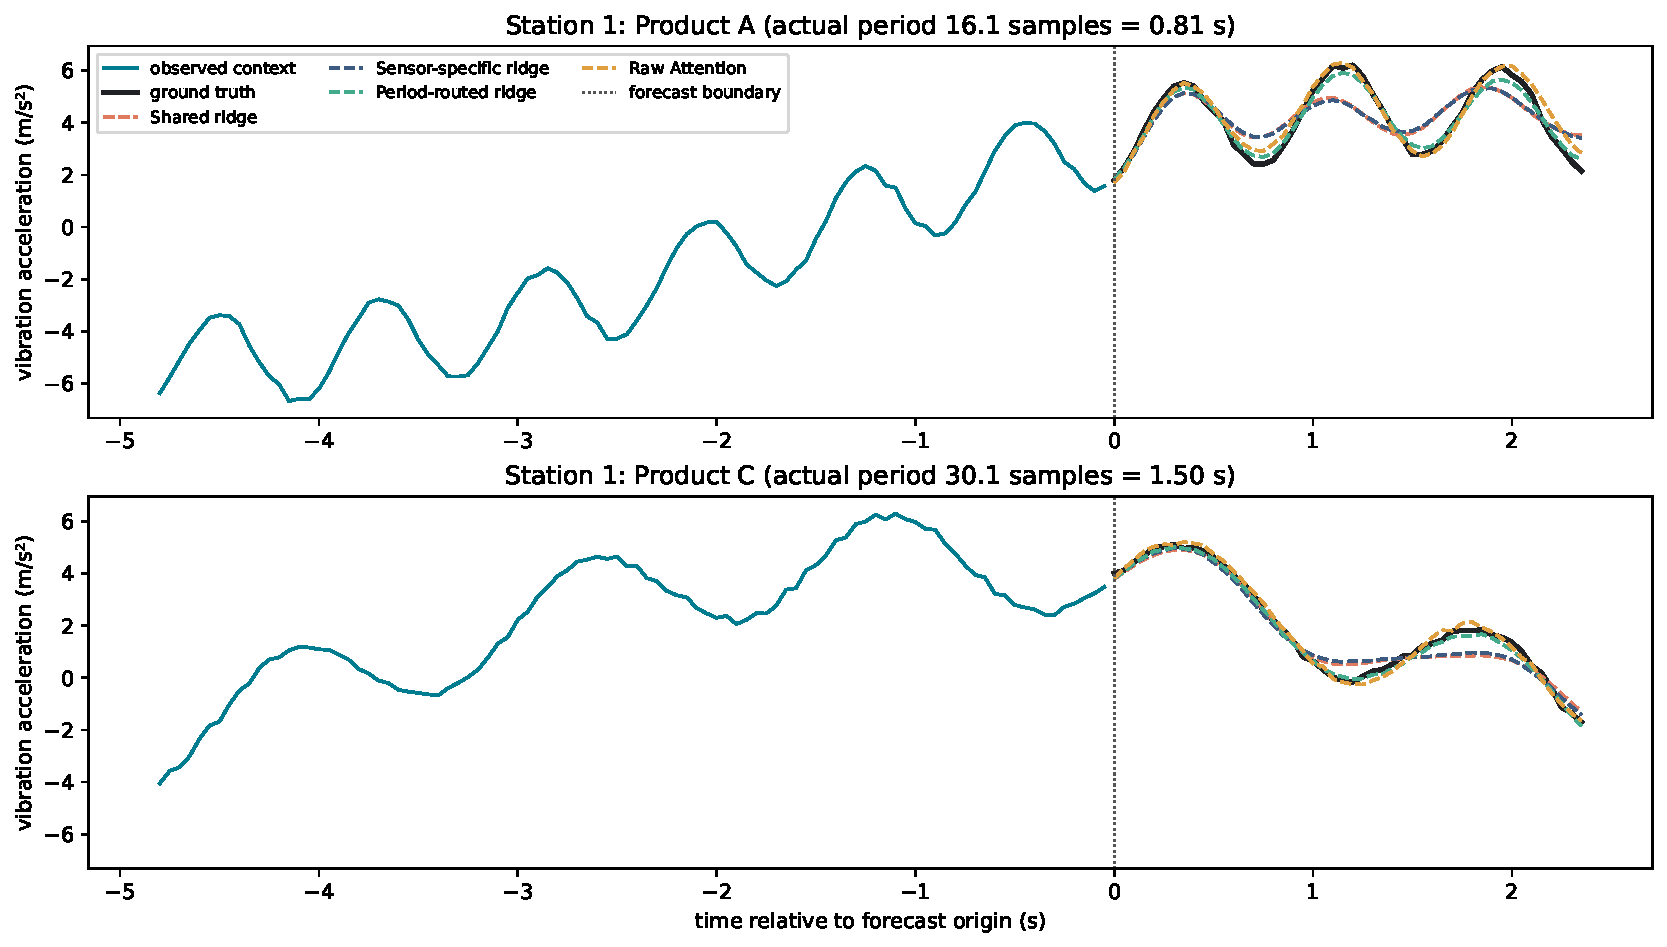
\includegraphics[width=0.95\textwidth]{figures/1.2-1.pdf}
\caption{Output 1.2: same station, two products.}
\end{figure}

Output 1.3 compares Attention weights for those two contexts. Mean absolute weight difference is about 0.012 and the max difference is about 0.43. So the same learned $W_Q,W_K,W_V$ produce different mixing for different inputs. Ridge cannot do that: $\hat W$ is fixed after fitting. I am not reading Output 1.3 as ``Attention found the physical period.'' It only shows that mixing depends on context.

\begin{figure}[H]
\centering
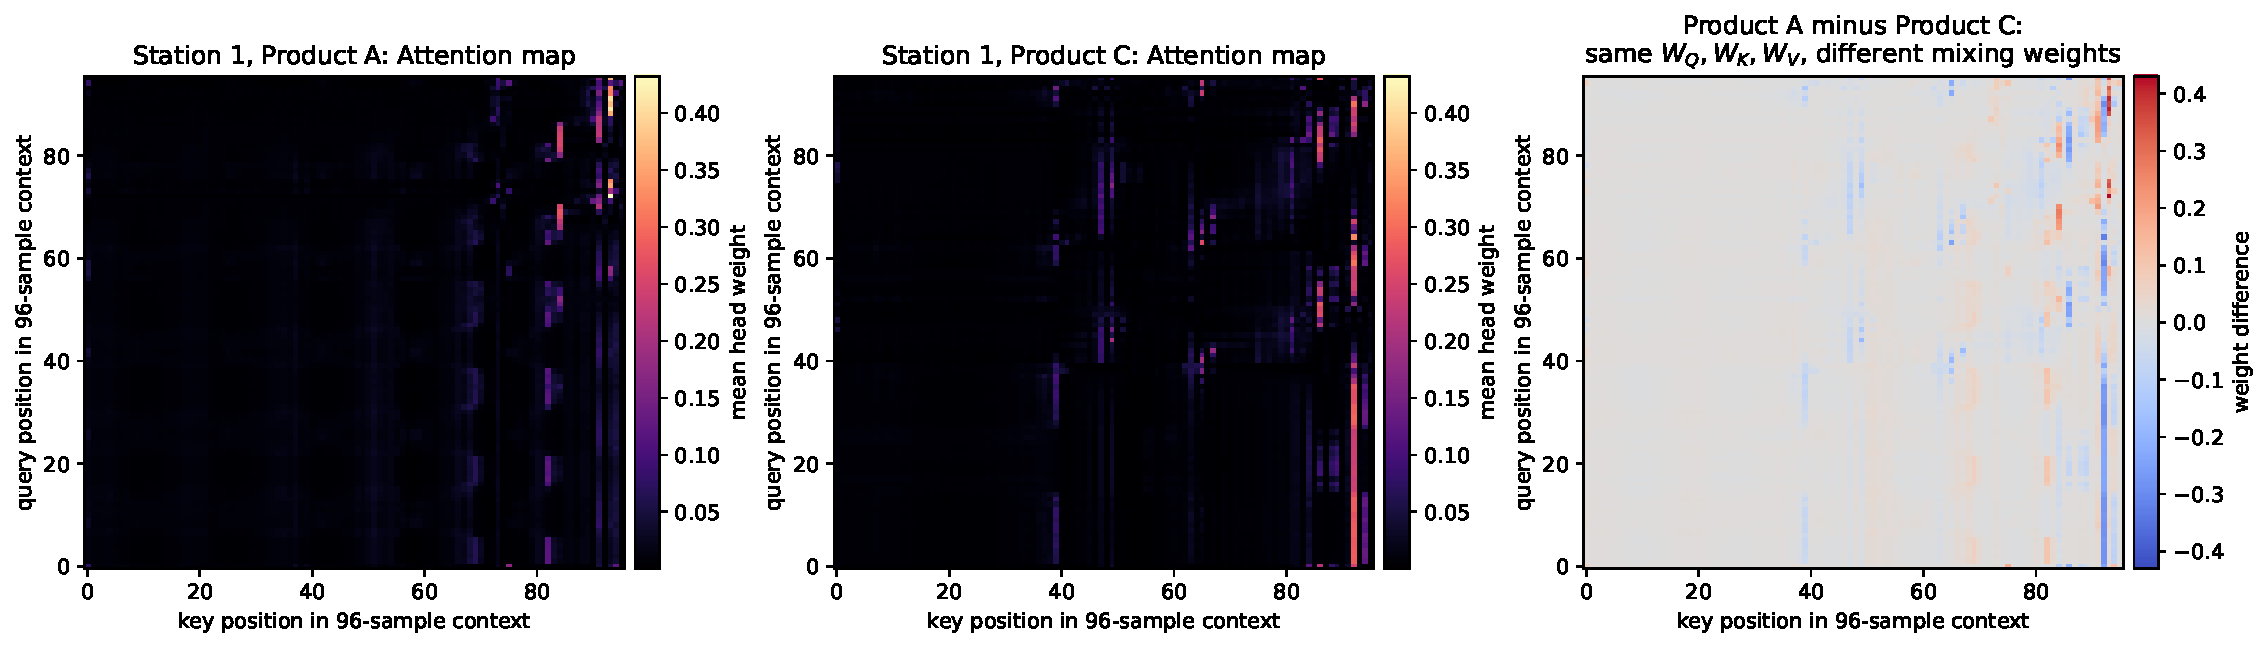
\includegraphics[width=0.95\textwidth]{figures/1.3-1.pdf}
\caption{Output 1.3: Attention weight difference across two contexts.}
\end{figure}

\section{Response 2}
I implemented centered moving-average decomposition with replicate padding at the ends.

Selected width: \textbf{41} (from Outputs 2.1--2.2). Wider widths push more energy into the residual and improve oracle period recovery. Width 41 has the highest recovery within one sample (0.998) among the candidates. Visually in Output 2.1, width 41 leaves a residual with clearer oscillation and a smoother trend than width 17.

\begin{figure}[H]
\centering
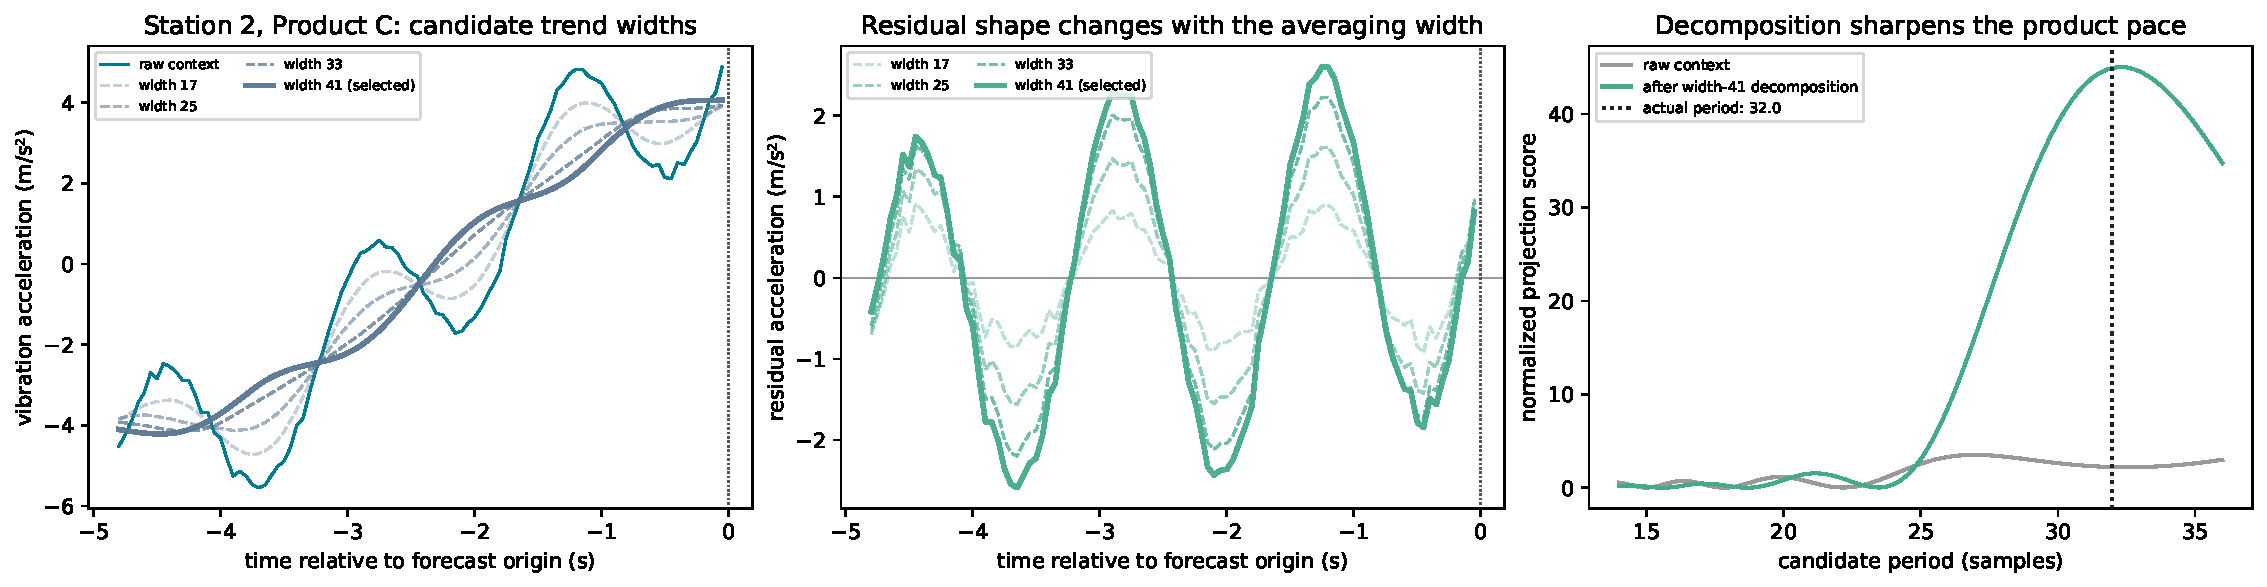
\includegraphics[width=0.85\textwidth]{figures/2.1-1.pdf}
\caption{Output 2.1: trend/residual for candidate widths.}
\end{figure}

\begin{figure}[H]
\centering
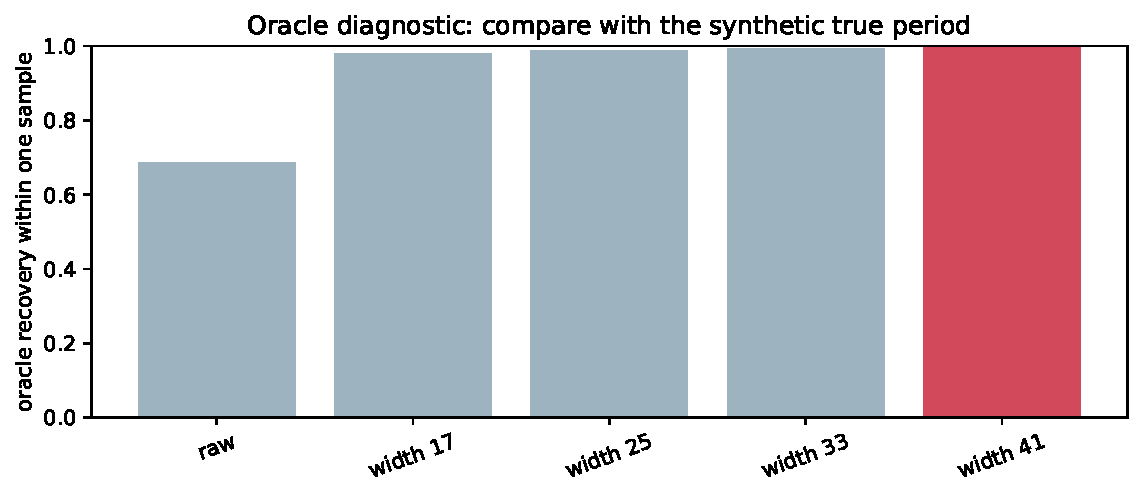
\includegraphics[width=0.7\textwidth]{figures/2.2-1.pdf}
\caption{Output 2.2: oracle period recovery vs width.}
\end{figure}

Output 2.3 (validation RMSE):
\begin{itemize}
  \item Established, Raw Attention $\approx 0.42$--$0.45$ by product.
  \item Established, Attention + decomposition $\approx 0.28$--$0.36$ by product.
\end{itemize}
So splitting helps. Held-out also improves (for example Product A: 0.64 $\to$ 0.40).

Why a moving average fits this world: drift is slow ($\sim$240 samples) and vibration is faster (14--36). A mid-range odd window can soak up the ramp while leaving most of the cycle in the remainder. The training-only oracle in Output 2.2 is useful because we can check whether the residual still reveals the known period before we trust the width for forecasting. It is not an input to the deployed model.

Where this bias fails: if the ``trend'' has a sharp step inside the context, a centered average smears the step into nearby samples and pollutes the residual. An alternative would be a causal low-pass filter (only past samples). That avoids peeking at future samples inside the window, but the edge behavior and phase lag would change.

\begin{figure}[H]
\centering
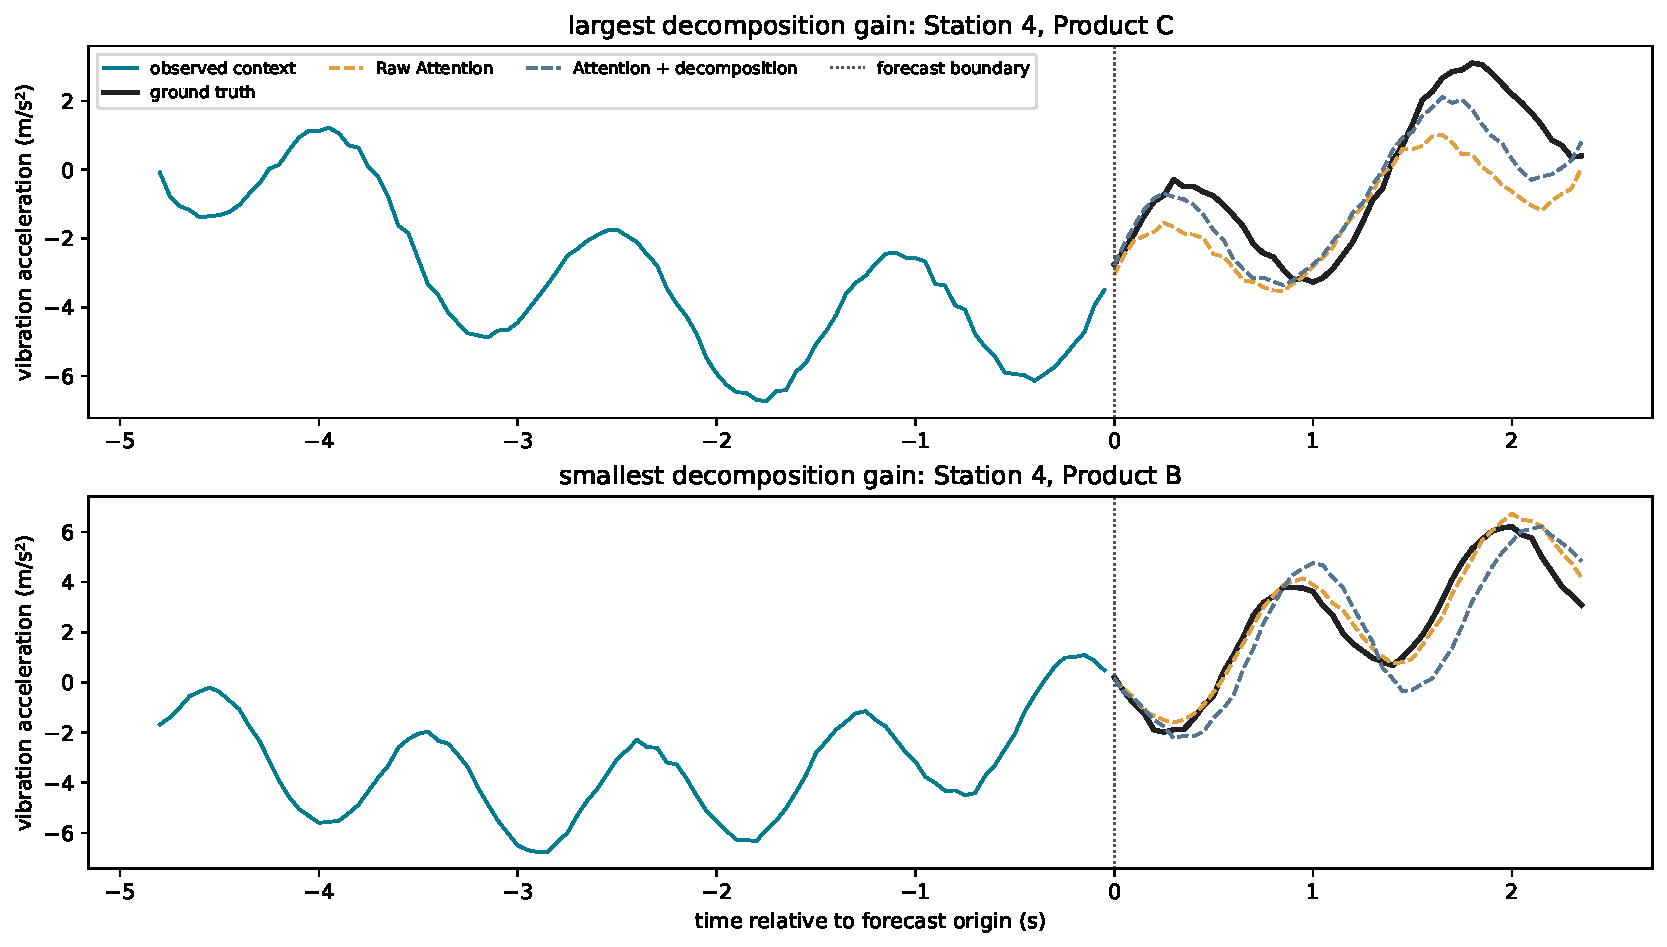
\includegraphics[width=0.85\textwidth]{figures/2.3-1.pdf}
\caption{Output 2.3: decomposition ablation forecasts.}
\end{figure}

\section{Response 3}
I implemented \texttt{aggregate\_delays}. The worked example with $v=[10,20,30,40]$, delays $[1,3]$, weights $[0.75,0.25]$ gives $z_0=35$, so the shift direction $(t-d)\bmod L$ is correct. Output 3.1 also matches FFT delay scores to the direct circular correlation on $[1,3,1,3]$.

Output 3.2 (signal-level diagnostic, not learned mixer scores): for Station 2, Product A, the strongest residual correlations sit at delay 16 and 32. The run period is $P\approx 16.13$, so those peaks are $P$ and $2P$.

\begin{figure}[H]
\centering
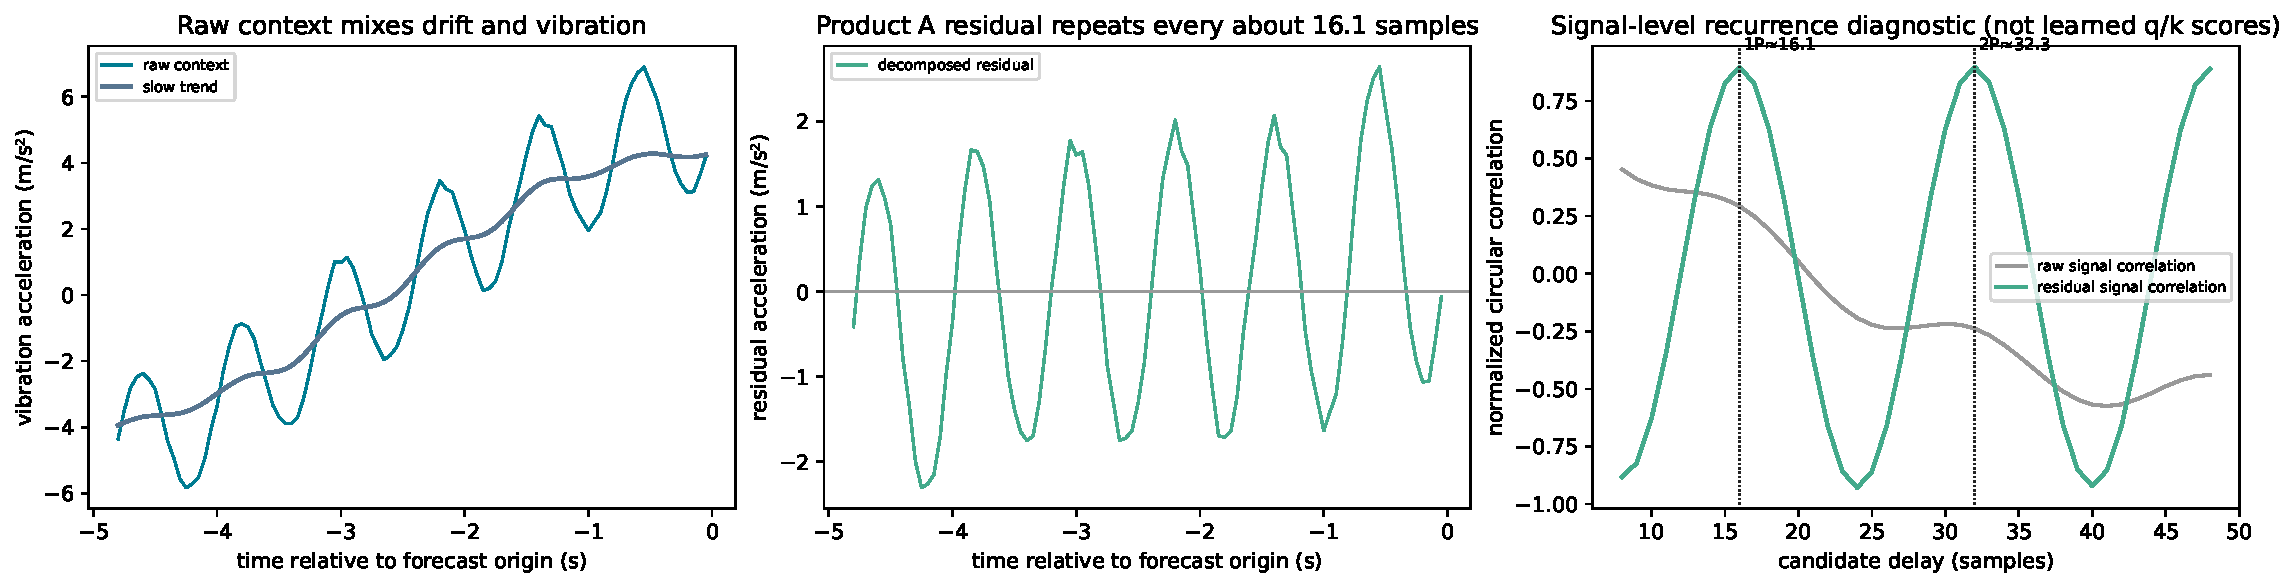
\includegraphics[width=0.75\textwidth]{figures/3.2-1.pdf}
\caption{Output 3.2: recurrence after removing slow structure.}
\end{figure}

Why decomposition helps delay evidence: a rising ramp looks similar to itself after many shifts, so raw circular correlation is muddy. After removing the slow part, peaks near $P$ and $2P$ stand out. That supports organizing mixing by a few recurring delays instead of every position pair.

When delay mixing is the wrong bias: a one-off transient (jam spike) that does not repeat inside the context. High scores would latch onto some lag that is not a real cycle, and the forecast would copy the wrong past segment.

\section{Response 4}
\subsection*{(a) Prediction before Output 4.1}
When the slow ramp is large, decomposition should help more than changing the mixer, because it sends the ramp to a linear trend head and keeps Attention/delay focused on the residual vibration.

\subsection*{(b) Four neural models and baselines (validation, established)}
\begin{table}[H]
\centering
\small
\begin{tabular}{lrrr}
\toprule
Model & RMSE & MSE & Fit s \\
\midrule
Period-routed ridge & 0.166 & 0.028 & 0.02 \\
Autoformer-inspired & 0.198 & 0.039 & 107 \\
Raw delay mixer & 0.220 & 0.048 & 90 \\
Attention + decomposition & 0.314 & 0.098 & 89 \\
Raw Attention & 0.430 & 0.184 & 75 \\
Shared ridge & 0.767 & 0.588 & 0.03 \\
\bottomrule
\end{tabular}
\caption{Output 4.1 / 1.1 validation on established stations.}
\end{table}

Switch effects from Raw Attention (0.430 RMSE): delay alone $\to$ 0.220; decomposition alone $\to$ 0.314; both $\to$ 0.198. The combined gain (0.232) is less than the sum of the separate gains (0.210+0.116=0.326), so the two upgrades overlap. Delay helps more than decomposition alone in this run. Output 4.2 shows RMSE rising with horizon for all models; period-routed ridge stays lowest across the 48 steps, and Autoformer-inspired is the best neural curve.

\begin{figure}[H]
\centering
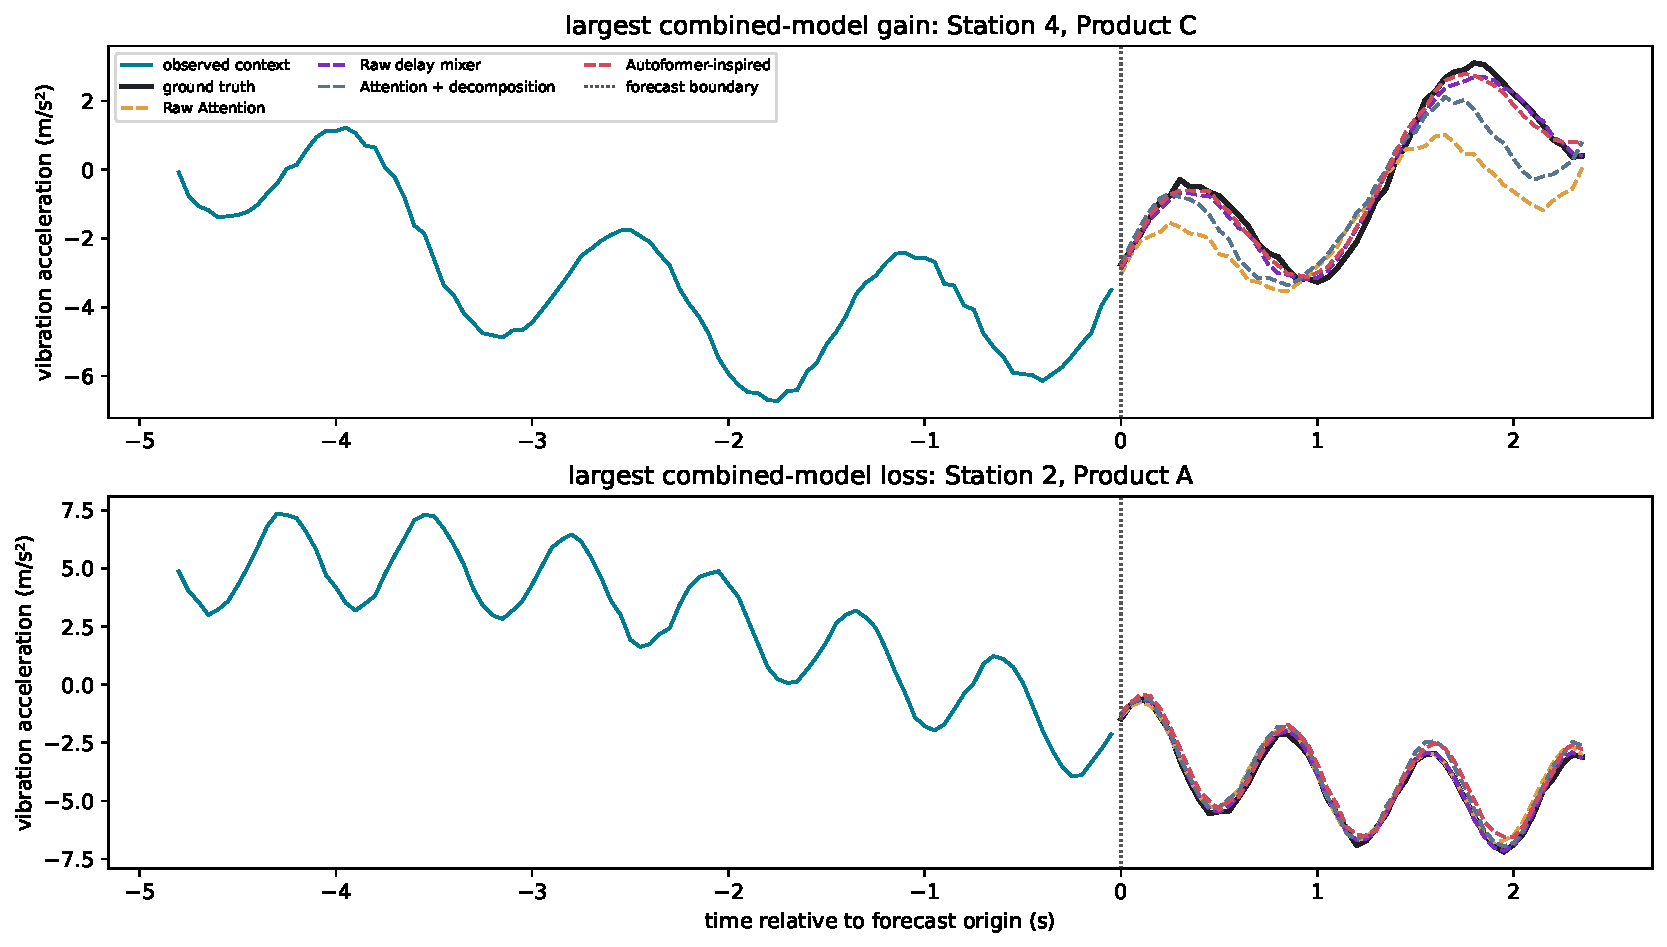
\includegraphics[width=0.95\textwidth]{figures/4.1-1.pdf}
\caption{Output 4.1: model comparison and example forecasts.}
\end{figure}

\begin{figure}[H]
\centering
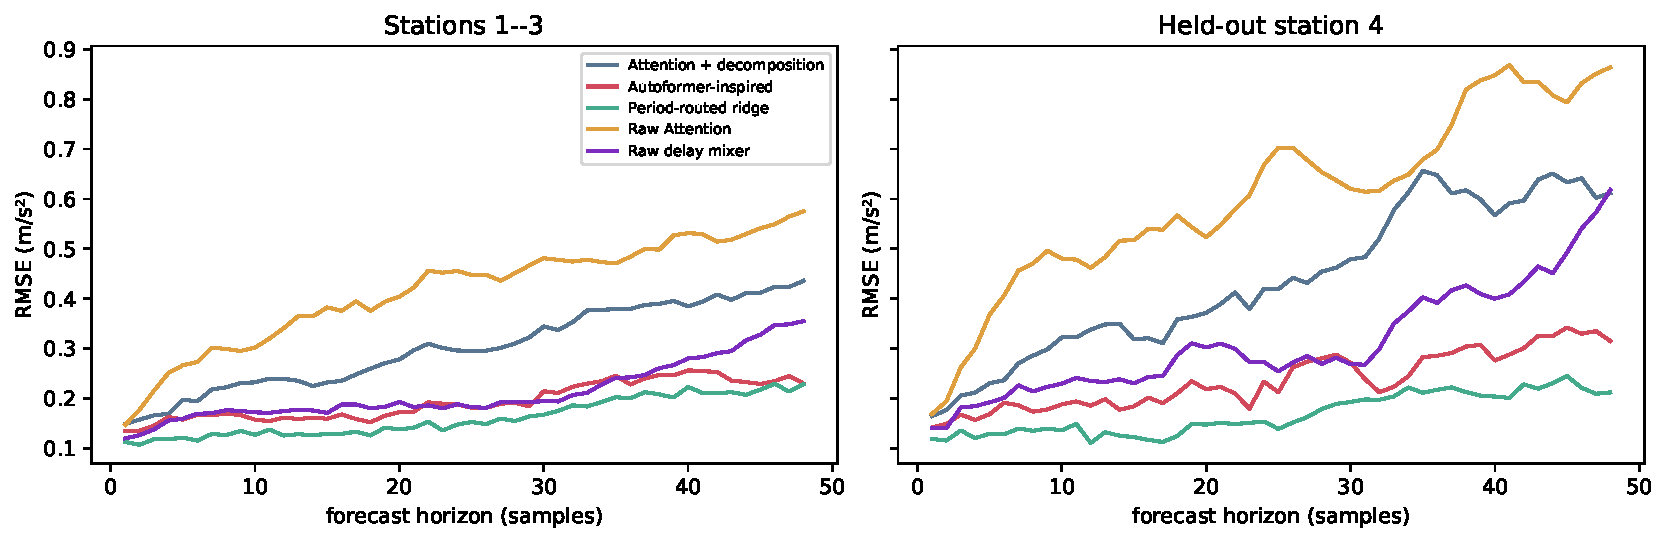
\includegraphics[width=0.95\textwidth]{figures/4.2-1.pdf}
\caption{Output 4.2: error vs forecast horizon.}
\end{figure}

\subsection*{(c) Deployment choices}
I deploy \textbf{Period-routed ridge} for established stations and for held-out station 4.
\begin{itemize}
  \item Best validation RMSE on both groups (0.166 and 0.173).
  \item Tiny cost: about 60k parameters and under 0.1 s fit, vs $\sim$370k parameters and $\sim$75--107 s for the neural models.
  \item Sensor-specific ridge is invalid for station 4.
\end{itemize}
Test check (Output 4.3): established test RMSE 0.161, held-out test RMSE 0.183. Close to validation, so the choice did not overfit the validation split.

\textbf{Response 4 interpretation (short).}
Both switches help, delay more than decomposition, and stacking them helps less than adding the two gains. Still, a linear model that is told the period beats every neural option here. Extra flexibility did not beat the right inductive bias on this benchmark.

\section*{AI use disclosure}
I used Cursor (Composer) while coding and while drafting this report.

\noindent\textbf{Coding prompts (summary):} implement the three TODO cells; fix local Jupyter/\texttt{ipykernel}; run the notebook on Colab with \texttt{PA1\_PRESET=full}; set up the GitHub repo.

\noindent\textbf{Model help on code:} filled \texttt{forward}, decomposition, and \texttt{aggregate\_delays}; helped with Colab execution and packaging.

\noindent\textbf{My edits on code:} checked shapes against the notebook contracts, kept the worked examples, chose width 41 and the period-routed deployment models from the validation tables myself.

\noindent\textbf{Report prompts (summary):} write Task 1 responses from the full-run CSVs/figures in simple English I can defend in a viva; avoid AI-sounding style.

\noindent\textbf{My edits on the report:} rewrote wording, cut fluff, kept only numbers from my \texttt{full} run, and matched each answer to the PDF response checklist.

\end{document}
